\chapter{Raíces de Ecuaciones y Sistemas No Lineales}
\section{Soluciones de las ecuaciones en una variable}
\subsection{El método de bisección}
Este proceso implica encontrar una raíz, o solución, para una ecuación de la forma $f(x) = 0$, para una función $f$ dada. Una raíz de esta ecuación también recibe el nombre de cero de la función $f$.

La primera técnica, basada en el teorema del valor intermedio, recibe el nombre de bisección, o método de búsqueda binaria.

Suponga que $f$ es una función continua definida dentro del intervalo $[a, b]$ con $f(a)$ y $f(b)$ de signos opuestos. El teorema del valor intermedio implica que existe un número $p$ en $(a, b)$ con $f(p) = 0$. A pesar de que el procedimiento operará cuando haya más de una raíz en el intervalo $(a, b)$, para simplicidad, nosotros asumimos que la raíz en este intervalo es única. El método realiza repetidamente una reducción a la mitad (o bisección) de los subintervalos de $[a, b]$ y, en cada paso, localizar la mitad que contiene $p$.

Para comenzar, sea $a_1 = a$ y $b_1 = b$ y sea $p_1$ es el punto medio de $[a, b]$, es decir,
\[p_1 = a_1 + \frac{b_1 - a_1}{2} = \frac{a_1 + b_1}{2}\]

\begin{itemize}
    \item Si $f(p_1) = 0$, entonces $p = p_1$ y terminamos.
    \item Si $f(p_1) \neq 0$, entonces $f(p_1)$ tiene el mismo signo que ya sea $f(a_1)$ o $f(b_1)$.
    \begin{itemize}
        \item Si $f(p_1)$ y $f(a_1)$ tienen el mismo signo, $p \in (p_1, b_1)$. Sea $a_2 = p_1$ y $b_2 = b_1$
        \item Si $f(p_1)$ y $f(a_1)$ tienen signos opuestos, $p \in (a_1, p_1)$. Sea $a_2 = a_1$ y $b_2 = p_1$.
    \end{itemize}
\end{itemize}

Entonces, volvemos a aplicar el proceso al intervalo $[a_2, b_2]$.

Se pueden aplicar otros procedimientos de parada, por ejemplo, podemos seleccionar una tolerancia $\epsilon > 0$ y generar $p_1, ..., p_N$ hasta que se cumpla una de las siguientes condiciones:
\begin{equation}
    |f(p_N)| < \epsilon
\end{equation}
\begin{equation}
    \frac{|p_N - p_{N-1|}}{|p_N|} < \epsilon, \quad p_N \neq 0
\end{equation}
\begin{equation}
    |p_N - p_{N-1}| < \epsilon
\end{equation}

El método de bisección, a pesar de que está conceptualmente claro, tiene desventajas significativas. Su velocidad de convergencia es más lenta y se podría descartar inadvertidamente una buena aproximación intermedia. Sin embargo, el método tiene la importante propiedad de que siempre converge a una solución y por esta razón con frecuencia se utiliza como iniciador para los métodos más eficientes que veremos más adelante en este capítulo.

\begin{theorem}
    Suponga que $f \in C[a, b]$ y $f(a) \cdot f(b) < 0$. El método de bisección genera una sucesión ${p_n}_{n = 1}^\infty$ que se aproxima a cero $p$ de $f$ con
    \[ |p_n - p| \leq \frac{b - a}{2^n} \text{, cuando } n \geq  1\]
\end{theorem}

\subsection{Iteración de punto fijo}
Un punto fijo para una función es un número en el que el valor de la función no cambia cuando se aplica la función.

\begin{definition}
    El número $p$ es un punto fijo para la función dada $g$ si $g(p) = p$.
\end{definition}

\begin{theorem}
    \begin{itemize}
        \item Si $g \in C[a, b]$ y $g(x) \in [a, b]$ para todas $x \in [a, b]$, entonces $g$ tiene por lo menos un punto fijo en $[a, b]$.
        \item Si, además, $g'(x)$ existe en $(a, b)$ y hay una constante positiva $k < 1$ con 
        \[ |g'(x)| \leq k, \forall x \in (a, b) \]
        entonces, existe exactamente un punto fijo en $[a, b]$. (Figura \ref{fig: Teorema del Punto Fijo})
    \end{itemize}
\end{theorem}

\begin{figure}[h]
    \centering
    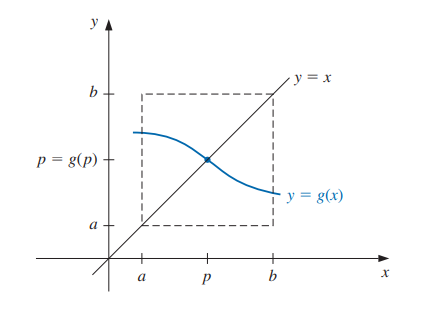
\includegraphics[width = 0.5 \textwidth]{Imagenes/6 - Teorema del Punto Fijo.png}
    \caption{Teorema del Punto Fijo}
    \label{fig: Teorema del Punto Fijo}
\end{figure}

\begin{proof}
    Si $g(a) = a$ o $g(b) = b$, entonces $g$ tiene un punto fijo en un extremo. De lo contrario, entonces $g(a) > a$ y $g(b) < b$. La función $h(x) = g(x) - x$ es continua en $[a, b]$, con
    \[h(a) = g(a) - a > 0 \quad \text{y} \quad h(b) = g(b) - b > 0 \]
    El teorema de valor intermedio implica que existe $p \in (a, b)$ para la cual $h(p) = 0$. Este número $p$ es un punto fijo para $g$ porque
    \[ 0 = h(p) = g(p) - p \quad \text{implica que} \quad g(p) = p\]

    Suponga, además, que $|g'(x)| \leq k < 1$ y que $p$ y $q$ son puntos fijos en $[a, b]$. Si $p \neq q$, entonces el teorema de valor medio implica que existe un número $\xi$ entre $p$ y $q$ y por lo tanto en $[a, b]$ con
    \[ \frac{g(p) - g(p)}{p - q} = g'(\xi)\]
    Por lo tanto
    \[ |p - q| = |g(p) - g(q)| = |g'(\xi)| |p - q| \leq k |p - q| < |p - q \]
    lo cual es una contradicción. Esta contradicción debe provenir de la única suposición $p \neq q$. Por lo tanto, $p = q$ y el punto fijo en $[a, b]$ es único.
\end{proof}

\subsubsection{Iteración de punto fijo}
Para aproximar el punto fijo de una función $g$, elegimos una aproximación inicial $p_0$ y generamos la sucesión ${p_n}_{n = 0}^\infty$ al permitir $p_n = g(p_{n-1})$, para cada $n \geq 1$. Si la sucesión converge a $p$ y $g$ es continua, entonces
\[p = \lim_{n \rightarrow \infty}{p_n} = \lim_{n \rightarrow \infty}{g (p_{n - 1})} = g \left( \lim_{n \rightarrow \infty}{p_{n - 1}} \right) = g(p)\]
y se obtiene una solución para $x = g(x)$. Esta técnica recibe el nombre de punto fijo o iteración funcional (Figura \ref{fig: Iteracion del Punto Fijo}).

\begin{figure}[h]
    \centering
    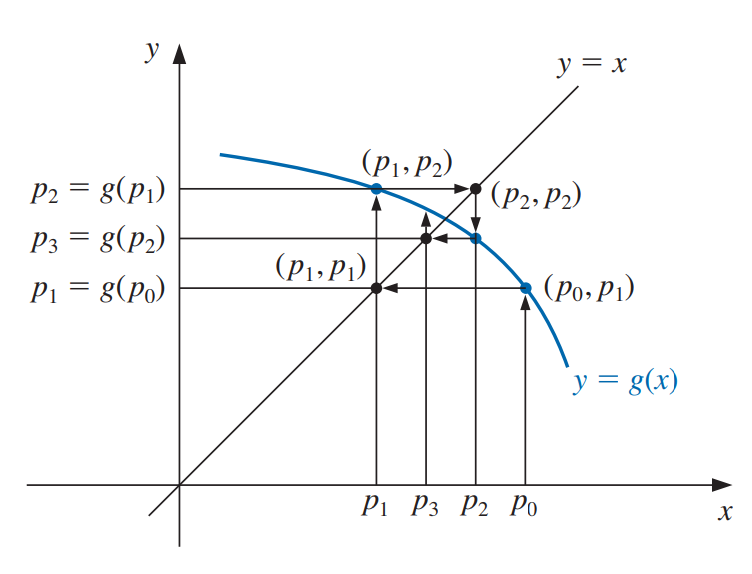
\includegraphics[width = 0.5 \textwidth]{Imagenes/6 - Iteracion del Punto Fijo a.png}
    \caption{Iteración del Punto Fijo}
    \label{fig: Iteracion del Punto Fijo}
\end{figure}

\begin{theorem}
    \label{Teorema de punto fijo}
    \textbf{(Teorema de punto fijo)} Sea $g \in C [a, b]$ tal que $g(x) \in [a, b]$ para todas las $x \in [a, b]$. Suponga, además, que existe $g'$ en $(a, b)$ y que existe una constante $0 < k < 1$ con
    \[ |g'(x)| \leq k, \text{ para todas } x \in (a, b) \]
    Entonces, para cualquier número $p_0$ en $[a, b]$, la sucesión definida por 
    \[ p_n = g(p_{n - 1}), \quad n \geq 1 \]
    converge al único punto fijo $p$ en $[a, b]$.
\end{theorem}

\begin{proof}
    El teorema \ref{Teorema de punto fijo} implica que existe un único punto $p$ en $[a, b]$ con $g(p) = p$. Ya que $g$ mapea $[a, b]$ en sí mismo, la sucesión ${p_n}_{n = 0}^\infty$ se define para todas las $n \geq 0$ y $p_n \in [a, b]$ para todas las $n$. Al utilizar el hecho de que $|g'(x)| \leq k|$ y el teorema de valor medio \ref{Teorema del valor medio}, tenemos, para cada $n$,
    \[ |p_n - p| = |g(p_{n - 1}) - g(p)| = |g'(\xi_n)| |p_{n - 1} - p| \leq k |p_{n - 1} - p| \]
    donde $\xi_n \in (a, b)$. Al aplicar esta desigualdad de manera inductiva obtenemos
    \begin{equation}
        |p_n - p| \leq k |p_{n - 1} - p| \leq k^2 |p_{n-2} - p| \leq ... \leq k^n |p_0 - p|\
    \end{equation}
    Ya que $0 < k < 1$, tenemos que $\lim_{n \rightarrow \infty}k^n = 0$ y
    \[ \lim_{n \rightarrow \infty} |p_n - p| \leq \lim_{n \rightarrow \infty} k^n |p_0 - p| = 0 \]
    Por lo tanto, ${p_n}_{n = 0}^\infty$ converge a $p$.
\end{proof}

\begin{remark}
    Si $g$ satisface las hipótesis del teorema \ref{Teorema de punto fijo}, entonces las octas del error relacionado con el uso de $p_n$ para aproximar $p$, están dadas por
    \begin{equation}
        |p_n - p| \leq k^n \max \left\{ p_0 - a, b - p_0 \right\}
    \end{equation}
    y
    \begin{equation}
        |p_n - p| \leq \frac{k^n}{1 - k}|p_1 - p_0|, \text{ para toda } n \geq 1
    \end{equation}
\end{remark}

\subsection{Método de Newton}

El método de Newton (o de Newton-Raphson) es uno de los métodos numéricos más poderosos y reconocidos para resolver un problema de encontrar la raíz. Existen muchas formas de presentar el método de Newton.

Supona que $f \in C^2[a, b]$. Si $p_0 \in [a, b]$ es una aproximación para $p$, de tal forma que $f'(p_0 \neq 0)$ y $|p - p_0|$ es ``pequeño''. Considere que el primer polinomio de Taylor para $f(x)$ expandido alrededor de $p_0$ y evaluado en $x = p$:

\[ f(p) = f(p_0) + (p - p_0)f'(p_0) + \frac{(p-p_0)^2}{2}f''(\xi(p)) \]

donde $\xi(p)$ se encuentra entre $p$ y $p_0$. Puesto que $f(p) = 0$, esta ecuación nos da
\[ 0 = f(p_0) + (p - p_0)f'(p_0) + \frac{(p-p_0)^2}{2}f''(\xi(p)) \]

El método de Newton se deriva al suponer que como $|p- p_0|$ es pequeño, el término relacionado con $(p - p_0)^2$ es mucho más pequeño, entonces

\[ 0 \approx f(p_0) + (p - p_0) f'(p_0)\]

Al resolver para $p$ obtenemos

\[ p \approx p_0 - \frac{f(p_0)}{f'(p_0)} \equiv p_1 \]

Esto constituye la base para el método de Newton, que empieza con una aproximación inicial $p_0$ y genera la sucesión ${p_n}_{n = 0}^\infty$, mediante

\begin{equation}
    \label{eq: Metodo de Newton}
    p_n = p_{n - 1} - \frac{f(p_{n - 1})}{f'(p_{n - 1})}, \text{ para } n \geq 1
\end{equation}

La figura \ref{fig: Metodo de Newton} ilustra cómo se obtienen las aproximaciones usando tangentes sucesivas.

\begin{figure}[h]
    \centering
    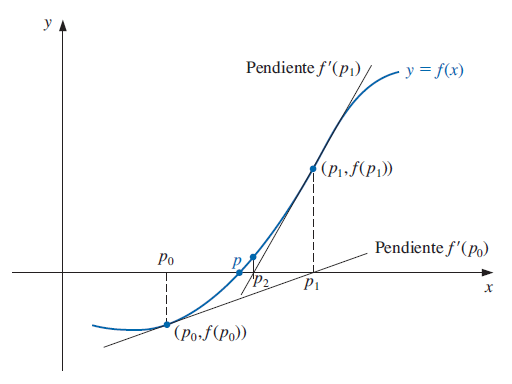
\includegraphics[width = 0.5 \textwidth]{Imagenes/6 - Metodo de Newton.png}
    \caption{Método de Newton}
    \label{fig: Metodo de Newton}
\end{figure}

\subsubsection{Convergencia con el método de Newton}

La derivación del método de Newton por medio de la serie de Taylor al inicio de la sección señala la importancia de una aproximación inicial precisa. La suposición crucial es que el término relacionado con $(p - p_0)^2$ es, en comparación con $|p - p_0|$, tan pequeño que se puede eliminar. Claramente esto será falso a menos que $p_0$ sea una buena aproximación para $p$. Si $p_0$ no está suficientemente cerca de la raíz real, existen pocas razones para sospechar que el método de Newton convergerá a la raíz. Sin embargo, en algunos casos, incluso las malas aproximaciones iniciales producirán convergencia.

\begin{theorem}
    \textbf{Teorema de Ostrowski.} Sea $f \in C^2 [a, b]$. Si $p \in (a, b)$ es tal que $f(p) = 0$ y $f'(p) \neq 0$, entonces existe una $\delta > 0$ tal que el método de Newton genera una sucesión ${p_n}_{n = 0}^\infty$ que converge a $p$ para cualquier aproximación inicial $p_0 \in [p - \delta, p + \delta]$.
\end{theorem}

\subsubsection{El método de la secante}

El método de Newton es una técnica en extremo poderosa, pero tiene una debilidad importante: la necesidad de conocer el valor de la derivada de $f$ en cada aproximación. Con frecuencia, $f'(x)$ es mucho más dificil y necesita más operaciones aritméticas para calcular $f(x)$. 

Para evitar el problema de la evaluación de la derivada en el método de Newton, presentamos una ligera variación. Por definición,
\[ f'(p_{n - 1}) = \lim_{x \rightarrow p_{n - 1}} \frac{f(x) - f(p_{n  - 1})}{x - p_{n  - 1}} \]
Si $p_{n - 2}$ está cerca de $p_{n - 1}$, Entonces
\[ f'(p_{n - 1}) \approx \frac{f(p_{n - 2}) - f(p_{n - 1})}{p_{n - 2} - p_{n - 1}} = \frac{f(p_{n - 1}) - f(p_{n - 2})}{p_{n - 1} - p_{n - 2}}\]
Usando esta aproximación para $f'(p_{n - 1})$ en la fórmula de Newton obtenemos
\begin{equation}
    \label{eq: Metodo de la secante}
    p_n = p_{n  - 1} - \frac{f(p_{n - 1}) (p_{n - 1} - p_{n - 2})}{f(p_{n - 1}) - f(p_{n - 2})}
\end{equation}

Esta técnica recibe el nombre de método de la secante y se ilustra en la figura \ref{fig: Metodo de la Secante}.

\begin{figure}[h]
    \centering
    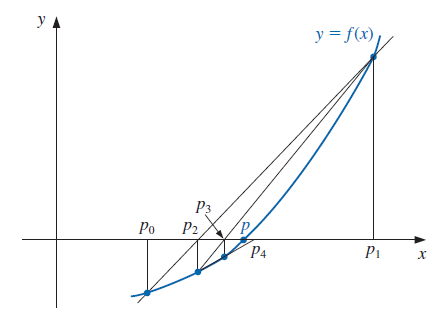
\includegraphics[width = 0.5 \textwidth]{Imagenes/6 - Metodo de la Secante.png}
    \caption{Método de la Secanta}
    \label{fig: Metodo de la Secante}
\end{figure}

\subsubsection{El método de posición falsa}

El método de posición falsa (también llamado Regula Falsi) genera aproximaciones de la misma manera que el método de la secante, pero incluye una prueba para garantizar que la raíz simepre se agrupa entre iteraciones sucesivas.

En primer lugar, seleccionamos las aproximaciones iniciales $p_0$ y $p_1$ con $f(p_0) \cdot f(p_1) < 0$. La aproximación $p_2$ se selecciona de la misma forma que en el método de la secante como la intersección en $x$ de la recta que une $(p_0, f(p_0))$ y $(p_1, f(p_1))$. Para decidir cuál línea secante se usa para calcular $p_3$, considere $f(p_2) \cdot f(p_1)$ o, más concretamente, $sgn f(p_2) \cdot sgn f(p_1)$ .
\begin{itemize}
    \item Si $sgn f(p_2) \cdot sgn f(p_1) < 0$, entonces $p_1$ y $p_2$ agrupan una raíz. Seleccione $p_3$ como la intersección en $x$ de la recta que une $(p_1, f(p_1))$ y $(p_2, f(p_2))$.
    \item Si no, seleccionamos $p_3$ como la intersección en $x$ de la recta que une $(p_0, f(p_0))$ y $(p_2, f(p_2))$ y, a continuación intercambia los índices en $p_0$ y $p_1$.
\end{itemize}

De manera similar, una vez se encuentra $p_3$, el signo de $f(p_3) \cdot f(p_2)$ determina si usamos $p_2$ y $p_3$ o $p_3$ y $p_1$ para calcular $p_4$. En el último caso, se vuelve a etiquetar $p_2$ y $p_1$. Reetiquetar garantiza que la raíz se agrupa entre iteraciones sucesivas. 

\begin{figure}[h]
    \centering
    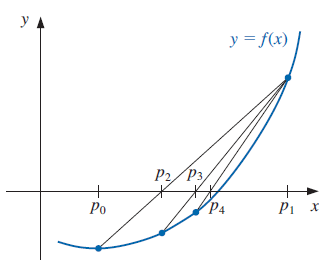
\includegraphics[width = 0.5 \textwidth]{Imagenes/6 - Metodo de Posicion Falsa.png}
    \caption{Método de la Posición Falsa}
    \label{fig: Metodo de la Posicion Falsa}
\end{figure}

\subsection{Análisis de error para métodos iterativos}
En esta sección inverstigamos el orden de convergencia de esquemas de iteración funcional y, con el propósito de obtener convergencia rápida, redescubrimo el método de Newton. También consideramos consideramos formas para acelerar la convergencia del método de Newton en circunstancias especiales. Primero, sin embargo, necesitamos un nuevo procedimiento para medir qué tan rápido converge una sucesión.

\subsubsection{Orden de convergencia}
\begin{definition}
    Suponga ${p_n}_{n = 0}^\infty$ es una sucesión que converge a $p$, con $p_n \neq p$ para todas las $n$. Si existen constantes positivas $\lambda$ y $\alpha$ con
    \[ \lim_{n \rightarrow \infty} \frac{|p_{n + 1} - p|}{|p_n - p|^\alpha} = \lambda \]
    Entonces ${p_n}_{n = 0}^\infty$ converge a $p$ de orden $\alpha$, con constante de error asintótica $\lambda$
\end{definition}

Se dice que una técnica iterativa de la forma $p_n = g(p_{n - 1})$ es de orden $\alpha$ si la sucesión ${p_n}_{n = 0}^\infty$ converge a la solución $p = g(p)$ de orden $\alpha$.

En general, una sucesión con un alto orden converge más rápidamente uqe una sucesión con un orden más bajo. La constante asintótica afecta la velocidad de concergencia pero no el grado del orden. Se presta atención especial a dos casos:
\begin{enumerate}
    \item Si $\alpha = 1$ (y $\lambda < 1$), la sucesión es linealmente convergente.
    \item Si $\alpha = 2$, la sucesión es cuadráticamente convergente.
\end{enumerate}

\begin{theorem}
    Sea $g \in [a, b]$ tal que $g(x) \in [a, b]$ para todas las $x \in [a, b]$. Suponga además que $g'$ es continua en $(a, b)$ y que existe una constante positiva $k < 1$ con 
    \[ |g'(x)| \leq k, \text{ para toda } x \in (a, b)\]
    Si $g'(p) \neq 0$, entonces para cualquier número $np_0 \neq p$ en $[a, b]$, la sucesión
    \[ p_n = g(p_{n - 1}), \text{ para } n \geq 1,\]
    Converge sólo linealmente para el único punto fijo $p$ en $[a, b]$.
\end{theorem}

\begin{proof}
    Sabemos que, a partir del teorema del punto fijo, la sucesión converge a $p$. Puesto que existe $g'$ en $(a, b)$, podemos aplicar el teorema del valor medio para $g$ para demostrar que para cualquier $n$,
    \[ p_{n + 1} - p = g(p_n) - g(p) = g'(\xi_n) (p_n - p) \]
    donde $\xi_n$ está entre $p_n$ y $p$. Ya que ${p_n}_{n = 0}^\infty$ converge a $p$, también tenemos que ${\xi_n}_{n = 0}^\infty$ converge a $p$. Puesto que $g_0$ es continua en $(a, b)$, tenemos
    \[ \lim_{n \rightarrow \infty} g'(\xi_n) = g'(p) \]
    Por lo tanto
    \[ \lim_{n \rightarrow \infty} \frac{p_{n + 1} - p}{p_n  - p} = \lim_{n \rightarrow \infty} g'(\xi_n) = g'(p) \]
    y
    \[ \lim_{n \rightarrow \infty} \frac{|p_{n + 1} - p|}{|p_n - p|} = |g'(p)|\]
    De este modo, si $|g'(p)| \neq 0$, la iteración de punto fijo muestra convergencia lineal con error asíntótico constante $|g'(p)|$.
\end{proof}

\begin{theorem}
    Sea $p$ una solución de la ecuación $x = g(x)$. Suponga que $g'(p) = 0$ y que $g''$ es continua con $|g''(x)| < M$ en un intervalo abierto $I$ que contiene a $p$. Entonces existe $\delta > 0$ talo que para $p_0 \in [p - \delta, p + \delta]$, la sucesión definida por $p_n = g(p_{n - 1})$, cuando $n \geq 1$, converge, por lo menos cuadráticamente a $p$. Además, con valores suficientemente grandes de n,
    \[ |p_{n + 1} - p| < \frac{M}{2} |p_n - p|^2 \]
\end{theorem}

\begin{proof}
    Seleccione $k$ en $(0,1)$ y $\delta > 0$ tal que el intervalo $[p - \delta, p + \delta]$, contenido en $I$, tenemos $|g'(x) \leq k$ y $g''$ continua.l Puesto que $|g'(x) \leq k < 1|$. Al expandir $g(x)$ en un polinomio lineal de Taylor, para $x \in [p - \delta, p + \delta]$ obtenemos
    \[ g(x) = g(p) + g'(p) (x - p) + \frac{g''(\xi)}{2} (x - p)^2 \]
    donde $\xi$ se encuentra entre $x$ y $p$. Las hipótesis $g(p) = p$ y $g'(p) = 0$ implican que 
    \[ g(x) = p + \frac{g''(\xi)}{2} (x - p)^2 \]
    En especial, cuando $x = p_n$,
    \[ p_{n + 1} = g(p_n) = p + \frac{g''(\xi_n)}{2} (p_n - p)^2 \]
    con $\xi_n$ entre $p_n$ y $p$. Por lo tanto,
    \[ p_{n + 1} - p = \frac{g''(\xi_n)}{2} (p_n - p)^2 \]
    Puesto que $|g'(x)| \leq k < 1$ en $[p - \delta, p + \delta]$ en sí mismo, por el teorema de putno fijo se sigue que ${p_n}_{n = 0}^\infty$ converge a $p$. Pero como $\xi_n$ se encuentra entre $p$ y $p_n$ para cada $n$, entonces ${\xi_n}_{n = 0}^\infty$ también converge a $p$ y
    \[ \lim_{n \rightarrow \infty} \frac{|p_{n + 1} - p|}{|p_n - p|^2} = \frac{|g''(p)|}{2} \]
    Este reseultado implica que la sucesión ${p_n}_{n = 0}^\infty$ es cuadráticamente convergente si $g''(p) \neq 0$ y de convergencia de orden superior si $g''(p) = 0$.

    Puesto que $g''$ es continua y está estrictamente acotada por $M$ en el intervalo $[p - \delta, p + \delta]$, esto también implica que, para los valores suficientemente grandes de $n$,
    \[ |p_{n + 1} - p| < \frac{M}{2} |p_n - p|^2 \]
\end{proof}

\subsubsection{Raíces múltiples}
\begin{definition}
    Una solución $p$ de $f(x) = 0$ es un cero de multiplicidad $m$ de $f$ si para $x \neq p$, podemos escribir $f(x) = (x - p)^m g(x)$, donde $\lim_{x \rightarrow p} g(x) \neq 0$.
\end{definition}

\begin{theorem}
    La función $f \in C^1[a, b]$ tiene un cero simple en $p$ en $(a, b)$ si y sólo si $f(p)= 0$, pero $f'(p) \neq 0$.
\end{theorem}

\begin{theorem}
    La función $f \in C^m[a, b]$ tiene un cero de multiplicidad $m$ en $p$ en $(a, b)$ si y sólo si
    \[ 0 = f(p) = f'(p) = f''(p) = ... = f^{(m - 1)(p)} \] 
    pero
    \[ f^{(m)}(p) \neq 0 \]
\end{theorem}

\section{Soluciones numéricas de sistemas de ecuaciones no lineales}

\subsection{Puntos fijos para funciones de varias variables}

Un sistema de ecuaciones no lineales tiene la forma
\begin{equation}
    \begin{cases}
        f_1 = (x_1 , x_2, ... , x_n) = 0 \\
        f_2 = (x_1 , x_2, ... , x_n) = 0 \\
        \quad \vdots \\
        f_2 = (x_1 , x_2, ... , x_n) = 0 \\
    \end{cases}
\end{equation}
donde cada función $f_i$ se puede pensar como un mapeo de un vector $x = (x_1, x_2, ..., x_n)^t$ del espacio $n$ dimensional $\mathbb{R}^n$ en la recta real $\mathbb{R}$

Este sistema de $n$ ecuaciones no lineales en $n$ variables también se puede representar al definir una función $F$ de mapeo $\mathbb{R}^n$ en $\mathbb{R}^n$.

Si se utiliza notacion vectorial para representar las variables $x_a, x_2, ...x_n$, entonces el sistema asume la forma
\begin{equation}
    F(x) = 0
\end{equation}

Las funciones $f_1, f_2, ..., f_n$ reciben el nombre de funciones coordenadas de $F$.

\begin{definition}
    Sea $f$ una función definida en un conjunto $D \subset \mathbb{R}^n$ en $\mathbb{R}$ y rango en $\mathbb{R}$. Se dice que la función $f$ tiene límite $L$ en $x_0$, escrito
    \[ \lim_{x \rightarrow x_0} f(x) = L \]
    si, dado cualquier número $\epsilon > 0$, existe un número $\delta > 0$ con
    \[ |f(x) - L| < \epsilon \]
    siempre que $x \in D$, y
    \[ 0 < \| x - x_0 \| < \delta \]
\end{definition}

\begin{definition}
    Sea $f$ una función del conjunto $D \subset \mathbb{R}^n$. La función $f$ es continua en $x_0 \in D$ siempre que exista $\lim_{x \rightarrow x_0} f(x_0)$ y 
    \[ \lim_{x \rightarrow x_0} f(x) = f(x_0) \]
    Además, $f$ es continua en un conjunto $D$ si $f$ es continua en cada punto de $D$. Este concepto se expresa al escribir $f \in C(D)$
\end{definition}

\begin{definition}
    Sea $F$ una función desde $D \subset \mathbb{R}^n$ a $\mathbb{R}^n$ de la forma
    \[ F(x) = (f_1(x), f_2(x), ..., f_n(x))^t \]
    donde $fi$ es un mapeo de $\mathbb{R}^n$ hasta $\mathbb{R}$ para cada $i$. Definimos
    \[ \lim_{x - x_0} F(x) = L = (L_1, L_2, ...L_n)^t \]
    si y sólo si $\lim_{x \rightarrow x_0} f_i(x) = L_i$ para cada $i = 1, 2, ..., n$.
\end{definition}

\begin{theorem}
    Sea $f$ una función de $D \subset \mathbb{R}^n$ a $\mathbb{R}$ y $x_0 \in D$. Suponga que existen todas las derivadas parciales de $f$ y las constantes $\delta > 0$ y $K > 0$, de tal forma que siempre que $\| x - x_0 \| < \delta $ y $x \in D$, tenemos
    \[ \left| \frac{\partial f(x)}{\partial x_j} \right| \leq K, \text{ para cada } j = 1, 2, ..., n\]
    Entonces $f$ es continua en $x_0$.
\end{theorem}

\subsubsection{Puntos fijos en $\mathbb{R}^n$}

\begin{definition}
    Una función $G$ desde $D \subset \mathbb{R}^n$ hasta $\mathbb{R}^n$ tiene un punto  fijo en $p \in D$ si $G(p) = p$.
\end{definition}

\begin{theorem}
    Sea $D = {(x_1, x_2, ..., x_n)^t | a_i \leq x_i \leq b_i, \text{ para cada } i = 1, 2, ..., n}$ para algún conjunto de constantes $a_1, a_2, ..., a_n$ y $b_1, b_2, ..., b_n$. Suponga que $G$ es una función continua en $D \subset \mathbb{R}^n$ a $\mathbb{R}$ con la propiedad de que $G(x) \in D$, siempre que $x \in D$. Entonces $G$ tiene un punto fijo en $D$.

    Además, suponga que todas las funciones componentes de $G$ tienen derivadas parciales continuas y que existe una constante $K < 1$ con
    \[ \left| \frac{\partial g_i(x)}{\partial x_j} \right| \leq G(x^{(k - 1)}), \quad \text{siempre que } x \in D \]
    para cada $j = 1, 2, ..., n$ y cada funcikón componente $g_i$. Entonces, la sucesión de punto fijo ${x^{(k)}}_{k = 0}^\infty$ definida por $x^{(0)}$ seleccionada arbitrariamente en $D$ y generada por medio de 
    \[ x^{(k)} = G(x^{(k - 1)}) \quad \text{para cada } k \geq 1 \]
    converge al único punto fijo $p \in D$ y 
    \begin{equation}
        \| x^{(k)} - p\|_\infty \leq \frac{K^k}{1 - K} \| x^{(1)} - x^{(0)} \|_\infty 
    \end{equation}
\end{theorem}

\subsection{Método de Newton}
Para construir el algoritmo que conduce a un método de punto fijo adecuado en el caso unidemnsional, encontramos una función $\phi$ con la proopiedad de que 
\[ g(x) = x - \phi(x) f(x) \]
da convergencia cuadrática para el punto fijo $p$ de la función $g$. A partir de esta condición el método de Newton evolucionó al seleccionar $\phi(x) = 1 / f'(x)$ suponiendo que $f'(x) \neq 0$.

Un enfoque similar en el caso $n$-dimensional implica una matriz
\begin{equation}
    A(x) = 
    \begin{bmatrix}
        a_{11}(x) & a_{12}(x) & \dots & a_{1n}(x) \\
        a_{21}(x) & a_{22}(x) & \dots & a_{2n}(x) \\
        \vdots & \vdots & & \vdots \\
        a_{n1}(x) & a_{n2}(x) & \dots & a_{nn}(x) \\
    \end{bmatrix}
\end{equation}
donde cada una de las entradas $a_{ij}(x)$ es una función de $\mathbb{R}^n$ a $\mathbb{R}$. Esto requiere encontrar $A(x)$ de tal forma que 
\[ G(x) = x - A(x)^{-1} F(x) \]
da convergencia cuadrática para la solución de $F(x) = 0$, suponiendo que $A(x)$ es no singular en el punto fijo $p$ de $G$.

\begin{theorem}
    \label{teo: Metodo de Newton Sistemas}
    Si $p$ es la solución de $G(x) = x$. Suponga que existe un número $\delta > 0$ con las propiedades:
    \begin{itemize}
        \item $\partial g_I / \partial x_j$ es continua en $N_\delta = {x | \|x - p\| < \delta}$, para cada $i = 1, 2, ..., n$ y $j = 1, 2, ..., n$
        \item $\partial^2g_i(x) / (\partial x_j \partial x_k)$ es continua y $| \partial^2g_i(x) / (\partial x_j \partial x_k) | \leq M$  para algunas constantes $M$, siempre que $x \in N_\delta$, para cada $i = 1, 2, ..., n$, $j = 1, 2, ..., n$ y $k = 1, 2, ..., n$.
        \item $\partial g_i(p) / \partial x_k = 0$, para cada $i = 1, 2, ..., n$ y $k = 1, 2, ..., n$.
    \end{itemize}
    Entonces, un número $\hat{\delta} \leq \delta$ existe de tal forma que la sucesión generada por $x^{(k)} = G(x^{(k - 1)})$ converge de forma cuadrática en $p$ para cualquier selección de $x^{(0)}$, siempre y cuando $\| x^{(0)} - p \| < \hat{\delta}$. Además,
    \[ \|x^{(k)} - p\|_\infty \leq \frac{n^2 M}{2} \| x^{(k - 1)} - p \|^2_\infty, \text{ para cada } k \geq 1 \]
\end{theorem}

\subsubsection{La matriz jacobiana}
Defina la matriz $J(x)$ mediante
\begin{equation}
    J(x) = 
    \begin{bmatrix}
        \frac{\partial f_1}{\partial x_1} (x) & \frac{\partial f_1}{\partial x_2} (x) & \dots & \frac{\partial f_1}{\partial x_n} (x) \\
        \frac{\partial f_2}{\partial x_1} (x) & \frac{\partial f_2}{\partial x_2} (x) & \dots & \frac{\partial f_2}{\partial x_n} (x) \\
        \vdots & \vdots & & \vdots \\
        \frac{\partial f_n}{\partial x_1} (x) & \frac{\partial f_n}{\partial x_2} (x) & \dots & \frac{\partial f_n}{\partial x_n} (x) \\
    \end{bmatrix}
\end{equation}

Una seleccion adecuada para $A(x)$ es $A(x) = J(x)$. La función $G$ se define mediante
\[ G(x) = x - J(x)^{-1} F(x) \]
y el procedimiento de iteración de punto fijo evoluciona al seleccionar $x^{(0)}$ y generar, para $k \geq 1$,
\begin{equation}
    x^{(k)} = G(x^{(k - 1)}) = x^{(k-1)} - J(x^{(k-1)})^{-1} F(x^{(k-1)})
\end{equation}

Esto recibe el nombre de método de Newton para sistemas no lineales y en general se espera que proporcione convergencia cuadrática, siempre y cuando se conozca un valor inicial suficientemente preciso y que $J(p)^{-1}$ exista.

Una debilidad en el método de Newton surge de la necesidad de calcular e invertir la matriz $J(x)$ en cada paso. En la práctica, el cálculo explícito de $J(x)^{-1}$ se evita al realizar la operación en una forma de dos pasos. Primero se encuentra un vector $y$ que satisface $J(x^{(k - 1)})y = -F(x^{(k - 1)})$. Entonces, la nueva aproximación, $x^{(k)}$, se obtiene sumando $y$ a $x^{(k - 1)}$.

\section*{Ejercicios}
\noindent (1) Calcular el número de iteraciones necesarias para aproximar la raíz del polinomio $p(x) = x^3 + x - 4$ en el intervalo $[1, 4]$ con el método de la Bisección.

\noindent (2) Calcular el número de iteraciones necesarias para aproximar la raíz del polinomio $p(x) = x^3 - x - 1$ en el intervalo $[1, 2]$ con el método de la Bisección.

\noindent (3) Probar que la función $g(x) = \pi + 0.5 sin(x/2)$ tiene un único punto fijo en el intervalo $[0, 2\pi]$.

\noindent (4) Probar que la función $q(x) = 2^{-x}$ tiene un único punto fijo en el intervalo $[1/3, 1]$.

\noindent (5) Encontrar una función de punto fijo para cada una de las siguientes funciones que converja a una raíz positiva:

a) $f(x) = 3 x^2 - e^x$

b) $f(x) = x - cos(x)$

\noindent (6) Analiza la convergencia del método del punto fijo $x_{k + 1} = g(x_k)$ para calcular los ceros $\alpha_1 = -1$ y $\alpha_2 = 2$ de la función $f(x) = x^2 - x - 2$ cuando se usan las funciones $g_1(x) = x^2 - 2$, $g_2(x) = \sqrt{2 + x}$, $g_3(x) = - \sqrt{2 + x}$, $g_4(x) = 1 + \frac{2}{x}$, $x \neq 0$.